\documentclass[a4paper,12pt]{article}

\usepackage[dutch]{babel}
\usepackage{fancyhdr}
\usepackage{graphicx}
\usepackage[pdftex,bookmarks=true]{hyperref}
\usepackage[utf8]{inputenc}
\usepackage{fullpage}
\usepackage{parskip}
\usepackage{float}
\usepackage{subcaption}
\usepackage{listings}
\usepackage{lscape}

\title{Samenvatting Databanken III - Hadoop \\ \large TIN 2 - HoGent}
\author{Lorenz Verschingel}

\begin{document}
\maketitle
\section{Intro to Hadoop}
\subsection{Core Hadoop components}
Hadoop is een project dat zich bezighoudt met het opslaan van data.
Deze manier van opslaan gebeurd in het Hadoop Distributed File System (HDFS).
Een manier om de data te verwerken is MapReduce.
Het hoofdconcept van Hadoop is dat de data opgesplitst wordt over verschillende machines, die een cluster genoemd worden.

\begin{figure}[H]
\centering
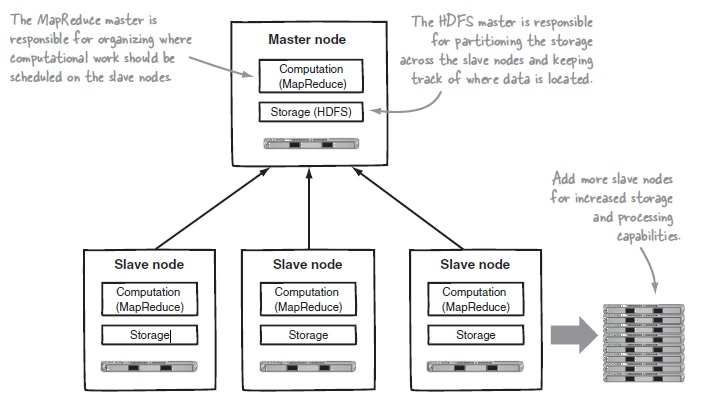
\includegraphics[scale=0.75]{img/HadoopCluster.jpg}
\caption{Cluster}
\label{hadoop-cluster}
\end{figure}

De verwerking van data gebeurd in waar de data opgeslagen is.

\subsection{Hadoop ecosystem}

\begin{figure}[H]
\centering
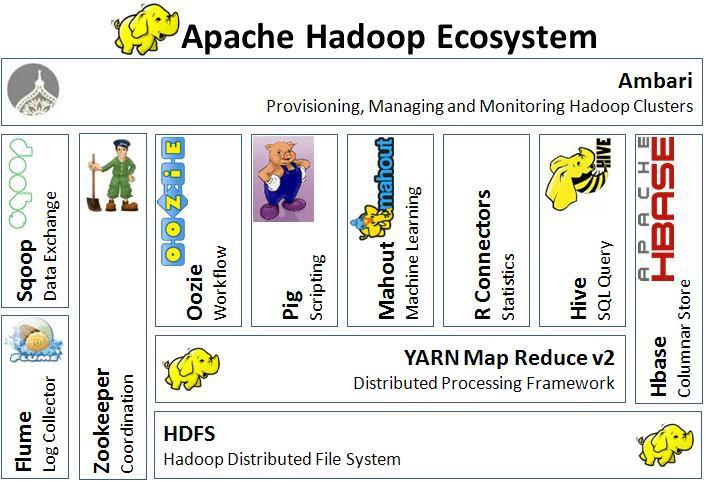
\includegraphics[scale=0.75]{img/HadoopEcosystem.jpg}
\caption{Hadoop Ecosystem}
\label{hadoop-ecosystem}
\end{figure}

\begin{itemize}
\item \textbf{HDFS}: Storage layer
\item \textbf{MapReduce}: Software layer die de verwerking doet
\item \textbf{Hive}: Zorgt ervoor dat HiveQL (gelijkend aan sql) wordt omgezet naar MapReduce
\item \textbf{HBase}: Zorgt voor random acces
\item \textbf{Mahout}: Data-mining
\item \textbf{Sqoop}: Exporteren en importeren naar relationele database
\item \textbf{Zookeeper}: Coördinatie
\end{itemize}

\subsection{Limitations}
\begin{enumerate}
\item \textbf{Availability}: Opgelost in Hadoop 2.x. Voordien single-master model $\rightarrow$ single-point of failure.
\item \textbf{Security}: default is het security model disabled, hierdoor is de enige beveiliging de ownership en permissions. Kerberos kan geïntegreerd worden.
\item \textbf{HDFS}: inefficiënt voor kleine files en geen transparante compressie.
\item \textbf{MapReduce}: batch-based $\rightarrow$ kan niet gebruikt worden voor real-time toepassingen
\item \textbf{Ecosystem versus compatibilities}: version-dependency challenges to running Hadoop
\end{enumerate}

\end{document}